%\documentclass[10pt]{beamer} % aspect ratio 4:3, 128 mm by 96 mm
\documentclass[10pt,aspectratio=169]{beamer} % aspect ratio 16:9
\graphicspath{{../../figures/}}
%\includeonlyframes{framezero,frameone,frametwo,framethree}
%%%%%%%%%%%%%%%%%%%%%%%%%%%%%%%%%%%%%%%%%%%%%%%%%%
% Packages
%%%%%%%%%%%%%%%%%%%%%%%%%%%%%%%%%%%%%%%%%%%%%%%%%%
\usepackage{appendixnumberbeamer}
\usepackage{booktabs}
\usepackage[scale=2]{ccicons}
\usepackage{pgfplots}
\usepackage{xspace}
\usepackage{amsmath}
\usepackage{totcount}
\usepackage{tikz}
%\usepackage{comment}
%\usetikzlibrary{external} % speedup compilation
%\tikzexternalize % activate!
%\usetikzlibrary{shapes,arrows}  

%\usepackage{bibentry}
%\nobibliography*
\usepackage{caption}%
\captionsetup[figure]{labelformat=empty}%
%%%%%%%%%%%%%%%%%%%%%%%%%%%%%%%%%%%%%%%%%%%%%%%%%%
% Metropolis theme custom modification file
%%%%%%%%%%%%%%%%%%%%%%%%%%%%%%%%%%%%%%%%%%%%%%%%%%
% Metropolis theme custom modification file
%%%%%%%%%%%%%%%%%%%%%%%%%%%%%%%%%%%%%%%%%%%%%%%%%%
% Metropolis theme custom colors
%%%%%%%%%%%%%%%%%%%%%%%%%%%%%%%%%%%%%%%%%%%%%%%%%%
\usetheme[progressbar=foot]{metropolis}
\useoutertheme{metropolis}
\useinnertheme{metropolis}
\usefonttheme{metropolis}
\setbeamercolor{background canvas}{bg=white}

%\usecolortheme{spruce}

\definecolor{myblue}{rgb}{0.19,0.55,0.91}
\definecolor{mediumblue}{rgb}{0,0,205}
\definecolor{darkblue}{rgb}{0,0,139}
\definecolor{Dodgerblue}{HTML}{1E90FF}
\definecolor{Navy}{HTML}{000080} % {rgb}{0,0,128}
\definecolor{Aliceblue}{HTML}{F0F8FF}
\definecolor{Lightskyblue}{HTML}{87CEFA}
\definecolor{logoblue}{RGB}{1,67,140}
\definecolor{Purple}{HTML}{911146}
\definecolor{Orange}{HTML}{CF4A30}

\setbeamercolor{progress bar}{bg=Lightskyblue}
\setbeamercolor{progress bar}{ fg=logoblue} 
\setbeamercolor{frametitle}{bg=logoblue}
\setbeamercolor{title separator}{fg=logoblue}
\setbeamercolor{block title}{bg=Lightskyblue!30,fg=black}
\setbeamercolor{block body}{bg=Lightskyblue!15,fg=black}
\setbeamercolor{alerted text}{fg=Purple}
%%%%%%%%%%%%%%%%%%%%%%%%%%%%%%%%%%%%%%%%%%%%%%%%%%
%  Theme modifications
%%%%%%%%%%%%%%%%%%%%%%%%%%%%%%%%%%%%%%%%%%%%%%%%%%
% modify progress bar linewidth
\makeatletter
\setlength{\metropolis@progressinheadfoot@linewidth}{2pt} 
\setlength{\metropolis@titleseparator@linewidth}{1pt}
\setlength{\metropolis@progressonsectionpage@linewidth}{1pt}

\setbeamertemplate{progress bar in section page}{
	\setlength{\metropolis@progressonsectionpage}{%
		\textwidth * \ratio{\thesection pt}{\totvalue{totalsection} pt}%
	}%
	\begin{tikzpicture}
	\fill[bg] (0,0) rectangle (\textwidth, \metropolis@progressonsectionpage@linewidth);
	\fill[fg] (0,0) rectangle (\metropolis@progressonsectionpage, \metropolis@progressonsectionpage@linewidth);
	\end{tikzpicture}%
}
\makeatother
\newcounter{totalsection}
\regtotcounter{totalsection}

\AtBeginDocument{%
	\pretocmd{\section}{\refstepcounter{totalsection}}{\typeout{Yes, prepending was successful}}{\typeout{No, prepending was not successful}}%
}%
%%%%%%%%%%%%%%%%%%%%%%%%%%%%%%%%%%%%%%%%%%%%%%%%%%
%  Bibliography mods
%%%%%%%%%%%%%%%%%%%%%%%%%%%%%%%%%%%%%%%%%%%%%%%%%%
\setbeamertemplate{bibliography item}{\insertbiblabel} %% Remove book symbol from references and add number in square brackets
% kill the abominable icon (without number)
%\setbeamertemplate{bibliography item}{}
%\makeatletter
%\renewcommand\@biblabel[1]{#1.} % number only
%\makeatother
% remove line breaks in bibliography
\setbeamertemplate{bibliography entry title}{}
\setbeamertemplate{bibliography entry location}{}
%%%%%%%%%%%%%%%%%%%%%%%%%%%%%%%%%%%%%%%%%%%%%%%%%%
%  Bibliography custom commands
%%%%%%%%%%%%%%%%%%%%%%%%%%%%%%%%%%%%%%%%%%%%%%%%%%
\newcommand{\bibliotitlestyle}[1]{\textbf{#1}\par}

\newif\ifinbiblio
\newcounter{bibkey}
\newenvironment{biblio}[2][long]{%
    %\setbeamertemplate{bibliography item}{\insertbiblabel}
    \setbeamertemplate{bibliography item}{}% without numbers
	\setbeamerfont{bibliography item}{size=\footnotesize}
	\setbeamerfont{bibliography entry author}{size=\footnotesize}
	\setbeamerfont{bibliography entry title}{size=\footnotesize}
	\setbeamerfont{bibliography entry location}{size=\footnotesize}
	\setbeamerfont{bibliography entry note}{size=\footnotesize}
	\ifx!#2!\else%
	\bibliotitlestyle{#2}%
	\fi%
	\begin{thebibliography}{}%
		\inbibliotrue%
		\setbeamertemplate{bibliography entry title}[#1]%
	}{%
		\inbibliofalse%
		\setbeamertemplate{bibliography item}{}%
	\end{thebibliography}%
}

\newcommand{\biblioref}[5][short]{
	\setbeamertemplate{bibliography entry title}[#1]
	\stepcounter{bibkey}%
	\ifinbiblio%
	\bibitem{\thebibkey}%
	#2
	\newblock #4
	\ifx!#5!\else\newblock {\em #5}, #3 \fi%
	\else%
	\begin{biblio}{}
		\bibitem{\thebibkey}
		#2
		\newblock #4
		\ifx!#5!\else\newblock {\em #5}, #3\fi
	\end{biblio}
	\fi
}
%
%\newbibmacro*{hypercite}{%
%	\renewcommand{\@makefntext}[1]{\noindent\normalfont##1}%
%	\footnotetext{%
%		\blxmkbibnote{foot}{%
%			\printtext[labelnumberwidth]{%
%				\printfield{prefixnumber}%
%				\printfield{labelnumber}}%
%			\addspace
%			\fullcite{\thefield{entrykey}}}}}
%
%\DeclareCiteCommand{\hypercite}%
%{\usebibmacro{cite:init}}
%{\usebibmacro{hypercite}}
%{}
%{\usebibmacro{cite:dump}}
%
%% Redefine the \footfullcite command to use the reference number
%\renewcommand{\footfullcite}[1]{\cite{#1}\hypercite{#1}}
%%%%%%%%%%%%%%%%%%%%%%%%%%%%%%%%%%%%%%%%%%%%%%%%%%
% Custom commands
%%%%%%%%%%%%%%%%%%%%%%%%%%%%%%%%%%%%%%%%%%%%%%%%%%
% matrix command 
\newcommand{\matr}[1]{\mathbf{#1}} % bold upright (Elsevier, Springer)
%\newcommand{\matr}[1]{#1}          % pure math version
%\newcommand{\matr}[1]{\bm{#1}}     % ISO complying version
% vector command 
\newcommand{\vect}[1]{\mathbf{#1}} % bold upright (Elsevier, Springer)
% derivative upright command
\DeclareRobustCommand*{\drv}{\mathop{}\!\mathrm{d}}
% 
\newcommand{\themename}{\textbf{\textsc{metropolis}}\xspace}

%%%%%%%%%%%%%%%%%%%%%%%%%%%%%%%%%%%%%%%%%%%%%%%%%%
%  Title page options
%%%%%%%%%%%%%%%%%%%%%%%%%%%%%%%%%%%%%%%%%%%%%%%%%%
% \date{\today}
\date{}
%%%%%%%%%%%%%%%%%%%%%%%%%%%%%%%%%%%%%%%%%%%%%%%%%%
% option 1
%%%%%%%%%%%%%%%%%%%%%%%%%%%%%%%%%%%%%%%%%%%%%%%%%%
\title{Elastic constants identification of composite laminates by using Lamb wave dispersion curves and optimization methods}
\subtitle{Lamb-opt}
\author{\textbf{Paweł Kudela}\\Maciej Radzieński \\Tomasz Wandowski \\Piotr Fiborek}
% logo align to Institute 
\institute{Institute of Fluid Flow Machinery\\Polish Academy of Sciences \\ \vspace{-1.5cm}\flushright 
\includegraphics[width=4cm]{../images/logo/logo_eng_40mm.eps}}
%%%%%%%%%%%%%%%%%%%%%%%%%%%%%%%%%%%%%%%%%%%%%%%%%%
% option 2 - authors in one line
%%%%%%%%%%%%%%%%%%%%%%%%%%%%%%%%%%%%%%%%%%%%%%%%%%
%	\title{Elastic constants identification of composite laminates by using Lamb wave dispersion curves and optimization methods}
%	\subtitle{Lamb-opt}
%	\author{\textbf{Paweł Kudela}\textsuperscript{2}, Maciej Radzieński\textsuperscript{2}, Wiesław Ostachowicz\textsuperscript{2}, Zhibo Yang\textsuperscript{1} }
%	% logo align to Institute 
%	\institute{\textsuperscript{1}Xi'an Jiaotong University \\ \textsuperscript{2}Institute of Fluid Flow Machinery\\ \hspace*{1pt} Polish Academy of Sciences \\ \vspace{-1.5cm}\flushright 
\includegraphics[width=4cm]{../images/logo/logo_eng_40mm.eps}}
%%%%%%%%%%%%%%%%%%%%%%%%%%%%%%%%%%%%%%%%%%%%%%%%%%
% option 3 - multilogo vertical
%%%%%%%%%%%%%%%%%%%%%%%%%%%%%%%%%%%%%%%%%%%%%%%%%%
%\title{Elastic constants identification of composite laminates by using Lamb wave dispersion curves and optimization methods}
%\subtitle{Lamb-opt}
%	\author{\textbf{Paweł Kudela}\inst{1}, Maciej Radzieński\inst{1}, Wiesław Ostachowicz\inst{1}, Zhibo Yang\inst{2} }
%	% logo under Institute 
%	\institute%
%	{ 
%		\inst{1}%
%		Institute of Fluid Flow Machinery\\ \hspace*{1pt} Polish Academy of Sciences \\ 
\includegraphics[height=0.85cm]{../images/logo/logo_eng_40mm.eps} \\
%		\and
%		\inst{2}%
%	    Xi'an Jiaotong University \\ 
\includegraphics[height=0.85cm]{../images/logo/logo_box.eps}
%    }
% end od option 3
%%%%%%%%%%%%%%%%%%%%%%%%%%%%%%%%%%%%%%%%%%%%%%%%%%
%% option 4 - 3 Institutes and logos horizontal centered
%%%%%%%%%%%%%%%%%%%%%%%%%%%%%%%%%%%%%%%%%%%%%%%%%%
%\title{Elastic constants identification of composite laminates by using Lamb wave dispersion curves and optimization methods}
%\subtitle{Lamb-opt }
%\author{\textbf{Paweł Kudela}\textsuperscript{1}, Maciej Radzieński\textsuperscript{1}, Marco Miniaci\textsuperscript{2}, Zhibo Yang\textsuperscript{3} }
%
%\institute{ 
%\begin{columns}[T,onlytextwidth]
%	\column{0.39\textwidth}
%	\begin{center}
%		\textsuperscript{1}Institute of Fluid Flow Machinery\\ \hspace*{3pt}Polish Academy of Sciences
%	\end{center}
%	\column{0.3\textwidth}
%	\begin{center}
%		\textsuperscript{2}Zurich University
%	\end{center}
%	\column{0.3\textwidth}
%	\begin{center}
%		\textsuperscript{3}Xi'an Jiaotong University
%	\end{center}
%\end{columns}
%\vspace{6pt}
%% logos 
%\begin{columns}[b,onlytextwidth]
%	\column{0.39\textwidth}
%		\centering 
%		
\includegraphics[width=\mywidth,height=0.85cm,keepaspectratio]{../images/logo/logo_eng_40mm.eps}
%	\column{0.3\textwidth}
%		\centering 
%		
\includegraphics[width=\mywidth,height=0.85cm,keepaspectratio]{../images/logo/logo_box.eps}
%	\column{0.3\textwidth}
%		\centering 
%		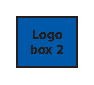
\includegraphics[width=\mywidth,height=0.85cm,keepaspectratio]{../images/logo/logo_box2.eps}
%\end{columns}
%}
%\makeatletter
%\setbeamertemplate{title page}{
%	\begin{minipage}[b][\paperheight]{\textwidth}
%		\centering  % <-- Center here
%		\ifx\inserttitlegraphic\@empty\else\usebeamertemplate*{title graphic}\fi
%		\vfill%
%		\ifx\inserttitle\@empty\else\usebeamertemplate*{title}\fi
%		\ifx\insertsubtitle\@empty\else\usebeamertemplate*{subtitle}\fi
%		\usebeamertemplate*{title separator}
%		\ifx\beamer@shortauthor\@empty\else\usebeamertemplate*{author}\fi
%		\ifx\insertdate\@empty\else\usebeamertemplate*{date}\fi
%		\ifx\insertinstitute\@empty\else\usebeamertemplate*{institute}\fi
%		\vfill
%		\vspace*{1mm}
%	\end{minipage}
%}
%
%\setbeamertemplate{title}{
%	%  \raggedright%  % <-- Comment here
%	\linespread{1.0}%
%	\inserttitle%
%	\par%
%	\vspace*{0.5em}
%}
%\setbeamertemplate{subtitle}{
%	%  \raggedright%  % <-- Comment here
%	\insertsubtitle%
%	\par%
%	\vspace*{0.5em}
%}
%\makeatother
% end of option 4
%%%%%%%%%%%%%%%%%%%%%%%%%%%%%%%%%%%%%%%%%%%%%%%%%%
% option 5 - 2 Institutes and logos horizontal centered
%%%%%%%%%%%%%%%%%%%%%%%%%%%%%%%%%%%%%%%%%%%%%%%%%%
%\title{Elastic constants identification of composite laminates by using Lamb wave dispersion curves and optimization methods}
%\subtitle{Lamb-opt }
%\author{\textbf{Paweł Kudela}\textsuperscript{1}, Maciej Radzieński\textsuperscript{1}, Marco Miniaci\textsuperscript{2}}
%
%\institute{ 
%	\begin{columns}[T,onlytextwidth]
%		\column{0.5\textwidth}
%			\centering
%			\textsuperscript{1}Institute of Fluid Flow Machinery\\ \hspace*{3pt}Polish Academy of Sciences
%		\column{0.5\textwidth}
%			\centering
%			\textsuperscript{2}Zurich University
%	\end{columns}
%	\vspace{6pt}
%	% logos 
%	\begin{columns}[b,onlytextwidth]
%		\column{0.5\textwidth}
%		\centering 
%		
\includegraphics[width=\mywidth,height=0.85cm,keepaspectratio]{../images/logo/logo_eng_40mm.eps}
%		\column{0.5\textwidth}
%		\centering 
%		
\includegraphics[width=\mywidth,height=0.85cm,keepaspectratio]{../images/logo/logo_box.eps}
%	\end{columns}
%}
%\makeatletter
%\setbeamertemplate{title page}{
%	\begin{minipage}[b][\paperheight]{\textwidth}
%		\centering  % <-- Center here
%		\ifx\inserttitlegraphic\@empty\else\usebeamertemplate*{title graphic}\fi
%		\vfill%
%		\ifx\inserttitle\@empty\else\usebeamertemplate*{title}\fi
%		\ifx\insertsubtitle\@empty\else\usebeamertemplate*{subtitle}\fi
%		\usebeamertemplate*{title separator}
%		\ifx\beamer@shortauthor\@empty\else\usebeamertemplate*{author}\fi
%		\ifx\insertdate\@empty\else\usebeamertemplate*{date}\fi
%		\ifx\insertinstitute\@empty\else\usebeamertemplate*{institute}\fi
%		\vfill
%		\vspace*{1mm}
%	\end{minipage}
%}
%
%\setbeamertemplate{title}{
%	%  \raggedright%  % <-- Comment here
%	\linespread{1.0}%
%	\inserttitle%
%	\par%
%	\vspace*{0.5em}
%}
%\setbeamertemplate{subtitle}{
%	%  \raggedright%  % <-- Comment here
%	\insertsubtitle%
%	\par%
%	\vspace*{0.5em}
%}
%\makeatother
% end of option 5
%
%%%%%%%%%%%%%%%%%%%%%%%%%%%%%%%%%%%%%%%%%%%%%%%%%%
%  End of title page options
%%%%%%%%%%%%%%%%%%%%%%%%%%%%%%%%%%%%%%%%%%%%%%%%%%
% logo option - alternative manual insertion by modification of coordinates in \put()
%\titlegraphic{%
%	%\vspace{\logoadheight}
%	\begin{picture}(0,0)
%	\put(305,-185){\makebox(0,0)[rb]{
\includegraphics[width=4cm]{../images/logo/logo_eng_40mm.eps}}}
%	\end{picture}}
%
%%%%%%%%%%%%%%%%%%%%%%%%%%%%%%%%%%%%%%%%%%%%%%%%%%
\AtBeginDocument{%
	%\def\myindenta{0.17\textwidth} % define myindenta variable  for correcting caption placement
	%\def\myindenta{0.18\textwidth} % 16:9 define myindenta variable  for correcting caption placement
	\def\myindenta{0.26\textwidth} % 4:3 define myindenta variable  for correcting caption placement
	\def\mywidtha{0.4\textwidth}  %16:9
	%\def\mywidtha{0.5\textwidth}  % 4:3
	\def\myindentb{0.05\textwidth} % define myindenta variable  for correcting caption placement
	\def\mywidthb{0.65\textwidth}  %16:9
	%\def\mywidthb{0.86\textwidth}  % 4:3
	\def\mywidthc{0.8\textwidth}  %16:9
	%\def\mywidthc{\textwidth}  % 4:3
	%\def\myindentc{0.12\textwidth} % 4:3 define myindenta variable  for correcting caption placement
	\def\myindentc{0.23\textwidth} % 16:9 define myindenta variable  for correcting caption placement
}%
%%%%%%%%%%%%%%%%%%%%%%%%%%%%%%%%%%%%%%%%%%%%%%%%%%
\begin{document}
%%%%%%%%%%%%%%%%%%%%%%%%%%%%%%%%%%%%%%%%%%%%%%%%%%
\maketitle
%%%%%%%%%%%%%%%%%%%%%%%%%%%%%%%%%%%%%%%%%%%%%%%%%%
% SLIDES
%%%%%%%%%%%%%%%%%%%%%%%%%%%%%%%%%%%%%%%%%%%%%%%%%%
\begin{frame}{Table of contents}
  \setbeamertemplate{section in toc}[sections numbered]
  \tableofcontents[hideallsubsections]
\end{frame}
%%%%%%%%%%%%%%%%%%%%%%%%%%%%%%%%%%%%%%%%%%%%%%%%%%
\section{Introduction}
%%%%%%%%%%%%%%%%%%%%%%%%%%%%%%%%%%%%%%%%%%%%%%%%%%
\begin{frame}[fragile,label=framezero]{Metropolis}

  The \themename theme is a Beamer theme with minimal visual noise
  inspired by the \href{https://github.com/hsrmbeamertheme/hsrmbeamertheme}{\textsc{hsrm} Beamer
  Theme} by Benjamin Weiss.

  Enable the theme by loading

  \begin{verbatim}    \documentclass{beamer}
    \usetheme{metropolis}\end{verbatim}

  Note, that you have to have Mozilla's \emph{Fira Sans} font and XeTeX
  installed to enjoy this wonderful typography.
\end{frame}
%%%%%%%%%%%%%%%%%%%%%%%%%%%%%%%%%%%%%%%%%%%%%%%%%%
\begin{frame}[fragile]{Sections}
  Sections group slides of the same topic

  \begin{verbatim}    \section{Elements}\end{verbatim}

  for which \themename provides a nice progress indicator \ldots
\end{frame}
%%%%%%%%%%%%%%%%%%%%%%%%%%%%%%%%%%%%%%%%%%%%%%%%%%
\section{Title formats}
%%%%%%%%%%%%%%%%%%%%%%%%%%%%%%%%%%%%%%%%%%%%%%%%%%
\begin{frame}{Metropolis titleformats}
	\themename supports 4 different titleformats:
	\begin{itemize}
		\item Regular
		\item \textsc{Smallcaps}
		\item \textsc{allsmallcaps}
		\item ALLCAPS
	\end{itemize}
	They can either be set at once for every title type or individually.
\end{frame}
%%%%%%%%%%%%%%%%%%%%%%%%%%%%%%%%%%%%%%%%%%%%%%%%%%
{
   % \metroset{titleformat frame=smallcaps}
\begin{frame}{Small caps}
	This frame uses the \texttt{smallcaps} titleformat.

	\begin{alertblock}{Potential Problems}
		Be aware, that not every font supports small caps. If for example you typeset your presentation with pdfTeX and the Computer Modern Sans Serif font, every text in smallcaps will be typeset with the Computer Modern Serif font instead.
	\end{alertblock}
\end{frame}
}
%%%%%%%%%%%%%%%%%%%%%%%%%%%%%%%%%%%%%%%%%%%%%%%%%%
{
%\metroset{titleformat frame=allsmallcaps}
\begin{frame}{All small caps}
	This frame uses the \texttt{allsmallcaps} titleformat.

	\begin{alertblock}{Potential problems}
		As this titleformat also uses smallcaps you face the same problems as with the \texttt{smallcaps} titleformat. Additionally this format can cause some other problems. Please refer to the documentation if you consider using it.

		As a rule of thumb: Just use it for plaintext-only titles.
	\end{alertblock}
\end{frame}
}
%%%%%%%%%%%%%%%%%%%%%%%%%%%%%%%%%%%%%%%%%%%%%%%%%%
{
%\metroset{titleformat frame=allcaps}
\begin{frame}{All caps}
	This frame uses the \texttt{allcaps} titleformat.

	\begin{alertblock}{Potential Problems}
		This titleformat is not as problematic as the \texttt{allsmallcaps} format, but basically suffers from the same deficiencies. So please have a look at the documentation if you want to use it.
	\end{alertblock}
\end{frame}
}
%%%%%%%%%%%%%%%%%%%%%%%%%%%%%%%%%%%%%%%%%%%%%%%%%%
\section{Elements}
%%%%%%%%%%%%%%%%%%%%%%%%%%%%%%%%%%%%%%%%%%%%%%%%%%
\begin{frame}[fragile]{Typography}
      \begin{verbatim}The theme provides sensible defaults to
\emph{emphasize} text, \alert{accent} parts
or show \textbf{bold} results.\end{verbatim}

  \begin{center}becomes\end{center}

  The theme provides sensible defaults to \emph{emphasize} text,
  \alert{accent} parts or show \textbf{bold} results.
\end{frame}
%%%%%%%%%%%%%%%%%%%%%%%%%%%%%%%%%%%%%%%%%%%%%%%%%%
\begin{frame}{Font feature test}
  \begin{itemize}
    \item Regular
    \item \textit{Italic}
    \item \textsc{SmallCaps}
    \item \textbf{Bold}
    \item \textbf{\textit{Bold Italic}}
    \item \textbf{\textsc{Bold SmallCaps}}
    \item \texttt{Monospace}
    \item \texttt{\textit{Monospace Italic}}
    \item \texttt{\textbf{Monospace Bold}}
    \item \texttt{\textbf{\textit{Monospace Bold Italic}}}
  \end{itemize}
\end{frame}
%%%%%%%%%%%%%%%%%%%%%%%%%%%%%%%%%%%%%%%%%%%%%%%%%%
\begin{frame}{Lists}
  \begin{columns}[T,onlytextwidth]
    \column{0.33\textwidth}
      Items
      \begin{itemize}
        \item Milk \item Eggs \item Potatos
      \end{itemize}

    \column{0.33\textwidth}
      Enumerations
      \begin{enumerate}
        \item First, \item Second and \item Last.
      \end{enumerate}

    \column{0.33\textwidth}
      Descriptions
      \begin{description}
        \item[PowerPoint] Meeh. \item[Beamer] Yeeeha.
      \end{description}
  \end{columns}
\end{frame}
\begin{frame}{Animation}
  \begin{itemize}[<+- | alert@+>]
    \item \alert<4>{This is\only<4>{ really} important}
    \item Now this
    \item And now this
  \end{itemize}
\end{frame}
%%%%%%%%%%%%%%%%%%%%%%%%%%%%%%%%%%%%%%%%%%%%%%%%%%
\begin{frame}[t]{SASE dispersion curves: density influence}
\vspace{-12pt} % 16:9
\begin{columns}[T]
	\column{0.5\textwidth}
	\newcommand{\modelname}{SASE2}
		\begin{figure}
			\only<1>{
			\includegraphics[width=\mywidthc]{SASE/\modelname_out/\modelname_angle_0_param_dispersion_curves.png}
			\caption{\hspace{\myindentc}The influence of \alert{matrix density}\\ \hspace{\myindentc}on dispersion curves at angle \textbf{0}$^{\circ}$}
			}
			\only<2>{
			\includegraphics[width=\mywidthc]{SASE/\modelname_out/\modelname_angle_15_param_dispersion_curves.png}
			\caption{\hspace{\myindentc}The influence of \alert{matrix density}\\ \hspace{\myindentc}on dispersion curves at angle \textbf{15}$^{\circ}$ }
			}
			\only<3>{
			\includegraphics[width=\mywidthc]{SASE/\modelname_out/\modelname_angle_30_param_dispersion_curves.png}
			\caption{\hspace{\myindentc}The influence of \alert{matrix density}\\ \hspace{\myindentc}on dispersion curves at angle \textbf{30}$^{\circ}$ }
			}
		    \only<4>{
		    	\includegraphics[width=\mywidthc]{SASE/\modelname_out/\modelname_angle_45_param_dispersion_curves.png}
		    	\caption{\hspace{\myindentc}The influence of \alert{matrix density}\\ \hspace{\myindentc}on dispersion curves at angle \textbf{45}$^{\circ}$ }
		    }
	    	\only<5>{
	    		\includegraphics[width=\mywidthc]{SASE/\modelname_out/\modelname_angle_60_param_dispersion_curves.png}
	    		\caption{\hspace{\myindentc}The influence of \alert{matrix density}\\ \hspace{\myindentc}on dispersion curves at angle \textbf{60}$^{\circ}$ }
	    	}
    		\only<6>{
    			\includegraphics[width=\mywidthc]{SASE/\modelname_out/\modelname_angle_75_param_dispersion_curves.png}
    			\caption{\hspace{\myindentc}The influence of \alert{matrix density}\\ \hspace{\myindentc}on dispersion curves at angle \textbf{75}$^{\circ}$ }
    		}
    		\only<7->{
    			\includegraphics[width=\mywidthc]{SASE/\modelname_out/\modelname_angle_90_param_dispersion_curves.png}
    			\caption{\hspace{\myindentc}The influence of \alert{matrix density}\\ \hspace{\myindentc}on dispersion curves at angle \textbf{90}$^{\circ}$ }
    		}
			\label{fig:rhom}
		\end{figure}
	\column{0.5\textwidth}
	\newcommand{\modelname}{SASE3}
		\begin{figure}
			\only<1>{
			\includegraphics[width=\mywidthc]{SASE/\modelname_out/\modelname_angle_0_param_dispersion_curves.png}
			\caption{\hspace{\myindentc}The influence of \alert{fibre density}\\ \hspace{\myindentc}on dispersion curves at angle \textbf{0}$^{\circ}$}
			}
			\only<2>{
			\includegraphics[width=\mywidthc]{SASE/\modelname_out/\modelname_angle_15_param_dispersion_curves.png}
			\caption{\hspace{\myindentc}The influence of \alert{fibre density}\\ \hspace{\myindentc}on dispersion curves at angle \textbf{15}$^{\circ}$}
			}
			\only<3>{
				\includegraphics[width=\mywidthc]{SASE/\modelname_out/\modelname_angle_30_param_dispersion_curves.png}
				\caption{\hspace{\myindentc}The influence of \alert{fibre density}\\ \hspace{\myindentc}on dispersion curves at angle \textbf{30}$^{\circ}$}
			}
			\only<4>{
				\includegraphics[width=\mywidthc]{SASE/\modelname_out/\modelname_angle_45_param_dispersion_curves.png}
				\caption{\hspace{\myindentc}The influence of \alert{fibre density}\\ \hspace{\myindentc}on dispersion curves at angle \textbf{45}$^{\circ}$}
			}
			\only<5>{
				\includegraphics[width=\mywidthc]{SASE/\modelname_out/\modelname_angle_60_param_dispersion_curves.png}
				\caption{\hspace{\myindentc}The influence of \alert{fibre density}\\ \hspace{\myindentc}on dispersion curves at angle \textbf{60}$^{\circ}$}
			}
			\only<6>{
				\includegraphics[width=\mywidthc]{SASE/\modelname_out/\modelname_angle_75_param_dispersion_curves.png}
				\caption{\hspace{\myindentc}The influence of \alert{fibre density}\\ \hspace{\myindentc}on dispersion curves at angle \textbf{75}$^{\circ}$}
			}
			\only<7->{
				\includegraphics[width=\mywidthc]{SASE/\modelname_out/\modelname_angle_90_param_dispersion_curves.png}
				\caption{\hspace{\myindentc}The influence of \alert{fibre density}\\ \hspace{\myindentc}on dispersion curves at angle \textbf{90}$^{\circ}$}
			}
			\label{fig:rhof}
		\end{figure}
\end{columns}
	\only<8>{
	\begin{alertblock}{Remarks}
		\textbf{Fibres density} has slightly more influence on dispersion curves than \textbf{matrix density}.
	\end{alertblock}
	}
\end{frame}
%%%%%%%%%%%%%%%%%%%%%%%%%%%%%%%%%%%%%%%%%%%%%%%%%%
\begin{frame}[t]{SASE dispersion curves: Young modulus influence}
\vspace{-12pt} % 16:9
\begin{columns}[T]
	\column{0.5\textwidth}
	\newcommand{\modelname}{SASE4}
	\begin{figure}
		\only<1>{
			\includegraphics[width=\mywidthc]{SASE/\modelname_out/\modelname_angle_0_param_dispersion_curves.png}
			\caption{\hspace{\myindentc}The influence of \alert{Young's modulus}\\ \hspace{\myindentc}\alert{of matrix} on dispersion curves at\\ \hspace{\myindentc}angle \textbf{0}$^{\circ}$}
		}
		\only<2>{
			\includegraphics[width=\mywidthc]{SASE/\modelname_out/\modelname_angle_15_param_dispersion_curves.png}
			\caption{\hspace{\myindentc}The influence of \alert{Young's modulus}\\ \hspace{\myindentc}\alert{of matrix} on dispersion curves at\\ \hspace{\myindentc}angle \textbf{15}$^{\circ}$ }
		}
		\only<3>{
			\includegraphics[width=\mywidthc]{SASE/\modelname_out/\modelname_angle_30_param_dispersion_curves.png}
			\caption{\hspace{\myindentc}The influence of \alert{Young's modulus}\\ \hspace{\myindentc}\alert{of matrix} on dispersion curves at\\ \hspace{\myindentc}angle \textbf{30}$^{\circ}$ }
		}
		\only<4>{
			\includegraphics[width=\mywidthc]{SASE/\modelname_out/\modelname_angle_45_param_dispersion_curves.png}
			\caption{\hspace{\myindentc}The influence of \alert{Young's modulus}\\ \hspace{\myindentc}\alert{of matrix} on dispersion curves at\\ \hspace{\myindentc}angle \textbf{45}$^{\circ}$ }
		}
		\only<5>{
			\includegraphics[width=\mywidthc]{SASE/\modelname_out/\modelname_angle_60_param_dispersion_curves.png}
			\caption{\hspace{\myindentc}The influence of \alert{Young's modulus}\\ \hspace{\myindentc}\alert{of matrix} on dispersion curves at\\ \hspace{\myindentc}angle \textbf{60}$^{\circ}$ }
		}
		\only<6>{
			\includegraphics[width=\mywidthc]{SASE/\modelname_out/\modelname_angle_75_param_dispersion_curves.png}
			\caption{\hspace{\myindentc}The influence of \alert{Young's modulus}\\ \hspace{\myindentc}\alert{of matrix} on dispersion curves at\\ \hspace{\myindentc}angle \textbf{75}$^{\circ}$ }
		}
		\only<7->{
			\includegraphics[width=\mywidthc]{SASE/\modelname_out/\modelname_angle_90_param_dispersion_curves.png}
			\caption{\hspace{\myindentc}The influence of \alert{Young's modulus}\\ \hspace{\myindentc}\alert{of matrix} on dispersion curves at\\ \hspace{\myindentc}angle \textbf{90}$^{\circ}$ }
		}
		\label{fig:em}
	\end{figure}
	\column{0.5\textwidth}
	\newcommand{\modelname}{SASE5}
	\begin{figure}
		\only<1>{
			\includegraphics[width=\mywidthc]{SASE/\modelname_out/\modelname_angle_0_param_dispersion_curves.png}
			\caption{\hspace{\myindentc}The influence of \alert{Young's modulus}\\ \hspace{\myindentc}\alert{of fibres} on dispersion curves at\\ \hspace{\myindentc}angle \textbf{0}$^{\circ}$}
		}
		\only<2>{
			\includegraphics[width=\mywidthc]{SASE/\modelname_out/\modelname_angle_15_param_dispersion_curves.png}
			\caption{\hspace{\myindentc}The influence of \alert{Young's modulus}\\ \hspace{\myindentc}\alert{of fibres} on dispersion curves at\\ \hspace{\myindentc}angle \textbf{15}$^{\circ}$}
		}
		\only<3>{
			\includegraphics[width=\mywidthc]{SASE/\modelname_out/\modelname_angle_30_param_dispersion_curves.png}
			\caption{\hspace{\myindentc}The influence of \alert{Young's modulus}\\ \hspace{\myindentc}\alert{of fibres} on dispersion curves at\\ \hspace{\myindentc}angle \textbf{30}$^{\circ}$}
		}
		\only<4>{
			\includegraphics[width=\mywidthc]{SASE/\modelname_out/\modelname_angle_45_param_dispersion_curves.png}
			\caption{\hspace{\myindentc}The influence of \alert{Young's modulus}\\ \hspace{\myindentc}\alert{of fibres} on dispersion curves at\\ \hspace{\myindentc}angle \textbf{45}$^{\circ}$}
		}
		\only<5>{
			\includegraphics[width=\mywidthc]{SASE/\modelname_out/\modelname_angle_60_param_dispersion_curves.png}
			\caption{\hspace{\myindentc}The influence of \alert{Young's modulus}\\ \hspace{\myindentc}\alert{of fibres} on dispersion curves at\\ \hspace{\myindentc}angle \textbf{60}$^{\circ}$}
		}
		\only<6>{
			\includegraphics[width=\mywidthc]{SASE/\modelname_out/\modelname_angle_75_param_dispersion_curves.png}
			\caption{\hspace{\myindentc}The influence of \alert{Young's modulus}\\ \hspace{\myindentc}\alert{of fibres} on dispersion curves at\\ \hspace{\myindentc}angle \textbf{75}$^{\circ}$}
		}
		\only<7->{
			\includegraphics[width=\mywidthc]{SASE/\modelname_out/\modelname_angle_90_param_dispersion_curves.png}
			\caption{\hspace{\myindentc}The influence of \alert{Young's modulus}\\ \hspace{\myindentc}\alert{of fibres} on dispersion curves at\\ \hspace{\myindentc}angle \textbf{90}$^{\circ}$}
		}
		\label{fig:ef}
	\end{figure}
\end{columns}
\only<8>{
	\begin{alertblock}{Remarks}
		\textbf{Young's modulus of matrix} has much more influence on dispersion curves than \textbf{Young's modulus of fibres}.
	\end{alertblock}
}
\end{frame}
%%%%%%%%%%%%%%%%%%%%%%%%%%%%%%%%%%%%%%%%%%%%%%%%%%
\begin{frame}[t,label=framethree]{SASE dispersion curves: Poisson's ratio influence}
\vspace{-12pt} % 16:9
\begin{columns}[T]
	\column{0.5\textwidth}
	\newcommand{\modelname}{SASE6}
	\begin{figure}
		\only<1>{
			\includegraphics[width=\mywidthc]{SASE/\modelname_out/\modelname_angle_0_param_dispersion_curves.png}
			\caption{\hspace{\myindentc}The influence of \alert{Poisson's ratio}\\ \hspace{\myindentc}\alert{of matrix} on dispersion curves at\\ \hspace{\myindentc}angle \textbf{0}$^{\circ}$}
		}
		\only<2>{
			\includegraphics[width=\mywidthc]{SASE/\modelname_out/\modelname_angle_15_param_dispersion_curves.png}
			\caption{\hspace{\myindentc}The influence of \alert{Poisson's ratio}\\ \hspace{\myindentc}\alert{of matrix} on dispersion curves at\\ \hspace{\myindentc}angle \textbf{15}$^{\circ}$ }
		}
		\only<3>{
			\includegraphics[width=\mywidthc]{SASE/\modelname_out/\modelname_angle_30_param_dispersion_curves.png}
			\caption{\hspace{\myindentc}The influence of \alert{Poisson's ratio}\\ \hspace{\myindentc}\alert{of matrix} on dispersion curves at\\ \hspace{\myindentc}angle \textbf{30}$^{\circ}$ }
		}
		\only<4>{
			\includegraphics[width=\mywidthc]{SASE/\modelname_out/\modelname_angle_45_param_dispersion_curves.png}
			\caption{\hspace{\myindentc}The influence of \alert{Poisson's ratio}\\ \hspace{\myindentc}\alert{of matrix} on dispersion curves at\\ \hspace{\myindentc}angle \textbf{45}$^{\circ}$ }
		}
		\only<5>{
			\includegraphics[width=\mywidthc]{SASE/\modelname_out/\modelname_angle_60_param_dispersion_curves.png}
			\caption{\hspace{\myindentc}The influence of \alert{Poisson's ratio}\\ \hspace{\myindentc}\alert{of matrix} on dispersion curves at\\ \hspace{\myindentc}angle \textbf{60}$^{\circ}$ }
		}
		\only<6>{
			\includegraphics[width=\mywidthc]{SASE/\modelname_out/\modelname_angle_75_param_dispersion_curves.png}
			\caption{\hspace{\myindentc}The influence of \alert{Poisson's ratio}\\ \hspace{\myindentc}\alert{of matrix} on dispersion curves at\\ \hspace{\myindentc}angle \textbf{75}$^{\circ}$ }
		}
		\only<7->{
			\includegraphics[width=\mywidthc]{SASE/\modelname_out/\modelname_angle_90_param_dispersion_curves.png}
			\caption{\hspace{\myindentc}The influence of \alert{Poisson's ratio}\\ \hspace{\myindentc}\alert{of matrix} on dispersion curves at\\ \hspace{\myindentc}angle \textbf{90}$^{\circ}$ }
		}
		\label{fig:nim}
	\end{figure}
	\column{0.5\textwidth}
	\newcommand{\modelname}{SASE7}
	\begin{figure}
		\only<1>{
			\includegraphics[width=\mywidthc]{SASE/\modelname_out/\modelname_angle_0_param_dispersion_curves.png}
			\caption{\hspace{\myindentc}The influence of \alert{Poisson's ratio}\\ \hspace{\myindentc}\alert{of fibres} on dispersion curves at\\ \hspace{\myindentc}angle \textbf{0}$^{\circ}$}
		}
		\only<2>{
			\includegraphics[width=\mywidthc]{SASE/\modelname_out/\modelname_angle_15_param_dispersion_curves.png}
			\caption{\hspace{\myindentc}The influence of \alert{Poisson's ratio}\\ \hspace{\myindentc}\alert{of fibres} on dispersion curves at\\ \hspace{\myindentc}angle \textbf{15}$^{\circ}$}
		}
		\only<3>{
			\includegraphics[width=\mywidthc]{SASE/\modelname_out/\modelname_angle_30_param_dispersion_curves.png}
			\caption{\hspace{\myindentc}The influence of \alert{Poisson's ratio}\\ \hspace{\myindentc}\alert{of fibres} on dispersion curves at\\ \hspace{\myindentc}angle \textbf{30}$^{\circ}$}
		}
		\only<4>{
			\includegraphics[width=\mywidthc]{SASE/\modelname_out/\modelname_angle_45_param_dispersion_curves.png}
			\caption{\hspace{\myindentc}The influence of \alert{Poisson's ratio}\\ \hspace{\myindentc}\alert{of fibres} on dispersion curves at\\ \hspace{\myindentc}angle \textbf{45}$^{\circ}$}
		}
		\only<5>{
			\includegraphics[width=\mywidthc]{SASE/\modelname_out/\modelname_angle_60_param_dispersion_curves.png}
			\caption{\hspace{\myindentc}The influence of \alert{Poisson's ratio}\\ \hspace{\myindentc}\alert{of fibres} on dispersion curves at\\ \hspace{\myindentc}angle \textbf{60}$^{\circ}$}
		}
		\only<6>{
			\includegraphics[width=\mywidthc]{SASE/\modelname_out/\modelname_angle_75_param_dispersion_curves.png}
			\caption{\hspace{\myindentc}The influence of \alert{Poisson's ratio}\\ \hspace{\myindentc}\alert{of fibres} on dispersion curves at\\ \hspace{\myindentc}angle \textbf{75}$^{\circ}$}
		}
		\only<7->{
			\includegraphics[width=\mywidthc]{SASE/\modelname_out/\modelname_angle_90_param_dispersion_curves.png}
			\caption{\hspace{\myindentc}The influence of \alert{Poisson's ratio}\\ \hspace{\myindentc}\alert{of fibres} on dispersion curves at\\ \hspace{\myindentc}angle \textbf{90}$^{\circ}$}
		}
		\label{fig:nif}
	\end{figure}
\end{columns}
\only<8>{
	\begin{alertblock}{Remarks}
		\textbf{Poisson's ratio of fibres} is the least influential parameter on dispersion curves among investigated parameters.
	\end{alertblock}
}
\end{frame}
%%%%%%%%%%%%%%%%%%%%%%%%%%%%%%%%%%%%%%%%%%%%%%%%%%
\begin{frame}[t,label=frameone]{SASE dispersion curves: volume fraction influence}
\vspace{-12pt} % 16:9
\newcommand{\modelname}{SASE8}
	\begin{figure}
		\only<1>{
			\includegraphics[width=\mywidtha]{SASE/\modelname_out/\modelname_angle_0_param_dispersion_curves.png}
			\caption{\hspace{\myindenta}The influence of \alert{volume fraction of reinforcing fibres}\\ \hspace{\myindenta}on dispersion curves at angle \textbf{0}$^{\circ}$}
		}
		\only<2>{
			\includegraphics[width=\mywidtha]{SASE/\modelname_out/\modelname_angle_15_param_dispersion_curves.png}
			\caption{\hspace{\myindenta}The influence of \alert{volume fraction of reinforcing fibres}\\ \hspace{\myindenta}on dispersion curves at angle \textbf{15}$^{\circ}$ }
		}
		\only<3>{
			\includegraphics[width=\mywidtha]{SASE/\modelname_out/\modelname_angle_30_param_dispersion_curves.png}
			\caption{\hspace{\myindenta}The influence of \alert{volume fraction of reinforcing fibres}\\ \hspace{\myindenta}on dispersion curves at angle \textbf{30}$^{\circ}$ }
		}
		\only<4>{
			\includegraphics[width=\mywidtha]{SASE/\modelname_out/\modelname_angle_45_param_dispersion_curves.png}
			\caption{\hspace{\myindenta}The influence of \alert{volume fraction of reinforcing fibres}\\ \hspace{\myindenta}on dispersion curves at angle \textbf{45}$^{\circ}$ }
		}
		\only<5>{
			\includegraphics[width=\mywidtha]{SASE/\modelname_out/\modelname_angle_60_param_dispersion_curves.png}
			\caption{\hspace{\myindenta}The influence of \alert{volume fraction of reinforcing fibres}\\ \hspace{\myindenta}on dispersion curves at angle \textbf{60}$^{\circ}$ }
		}
		\only<6>{
			\includegraphics[width=\mywidtha]{SASE/\modelname_out/\modelname_angle_75_param_dispersion_curves.png}
			\caption{\hspace{\myindenta}The influence of \alert{volume fraction of reinforcing fibres}\\ \hspace{\myindenta}on dispersion curves at angle \textbf{75}$^{\circ}$ }
		}
		\only<7->{
			\includegraphics[width=\mywidtha]{SASE/\modelname_out/\modelname_angle_90_param_dispersion_curves.png}
			\caption{\hspace{\myindenta}The influence of \alert{volume fraction of reinforcing fibres}\\ \hspace{\myindenta}on dispersion curves at angle \textbf{90}$^{\circ}$ }
		}
		\label{fig:vol}
	\end{figure}

\only<8>{
	\begin{alertblock}{Remarks}
		\textbf{Volume fraction} of reinforcing fibres is the most influential parameter on dispersion curves among investigated parameters.
	\end{alertblock}
}
\end{frame}
%%%%%%%%%%%%%%%%%%%%%%%%%%%%%%%%%%%%%%%%%%%%%%%%%%
\begin{frame}[t,label=frametwo]{Comparison of numerical and experimental dispersion curves}
\newcommand{\modelname}{SASE1}
\begin{figure}
	\only<1>{
		\includegraphics[width=\mywidthb]{SASE/\modelname_out/\modelname_25_angle_0_num_exp_dispersion.png}
		\caption{\hspace{\myindentb}Comparison of numerical and experimental dispersion curves at angle \textbf{0}$^{\circ}$}
	}
	\only<2>{
		\includegraphics[width=\mywidthb]{SASE/\modelname_out/\modelname_25_angle_15_num_exp_dispersion.png}
		\caption{\hspace{\myindentb}Comparison of numerical and experimental dispersion curves at angle \textbf{15}$^{\circ}$ }
	}
	\only<3>{
		\includegraphics[width=\mywidthb]{SASE/\modelname_out/\modelname_25_angle_30_num_exp_dispersion.png}
		\caption{\hspace{\myindentb}Comparison of numerical and experimental dispersion curves at angle \textbf{30}$^{\circ}$ }
	}
	\only<4>{
		\includegraphics[width=\mywidthb]{SASE/\modelname_out/\modelname_25_angle_45_num_exp_dispersion.png}
		\caption{\hspace{\myindentb}Comparison of numerical and experimental dispersion curves at angle \textbf{45}$^{\circ}$ }
	}
	\only<5>{
		\includegraphics[width=\mywidthb]{SASE/\modelname_out/\modelname_25_angle_60_num_exp_dispersion.png}
		\caption{\hspace{\myindentb}Comparison of numerical and experimental dispersion curves at angle \textbf{60}$^{\circ}$ }
	}
	\only<6>{
		\includegraphics[width=\mywidthb]{SASE/\modelname_out/\modelname_25_angle_75_num_exp_dispersion.png}
		\caption{\hspace{\myindentb}Comparison of numerical and experimental dispersion curves at angle \textbf{75}$^{\circ}$ }
	}
	\only<7>{
		\includegraphics[width=\mywidthb]{SASE/\modelname_out/\modelname_25_angle_90_num_exp_dispersion.png}
		\caption{\hspace{\myindentb}Comparison of numerical and experimental dispersion curves at angle \textbf{90}$^{\circ}$ }
	}
	\label{fig:numexp}
\end{figure}
\end{frame}

%%%%%%%%%%%%%%%%%%%%%%%%%%%%%%%%%%%%%%%%%%%%%%%%%%
\begin{frame}{Tables}
  \begin{table}
    \caption{Largest cities in the world (source: Wikipedia)}
    \begin{tabular}{lr}
      \toprule
      City & Population\\
      \midrule
      Mexico City & 20,116,842\\
      Shanghai & 19,210,000\\
      Peking & 15,796,450\\
      Istanbul & 14,160,467\\
      \bottomrule
    \end{tabular}
  \end{table}
\end{frame}
%%%%%%%%%%%%%%%%%%%%%%%%%%%%%%%%%%%%%%%%%%%%%%%%%%
\begin{frame}{Tables cd}
\begin{table}
	\label{tab:mat_prop}
	\renewcommand{\arraystretch}{1.3}
	\centering \footnotesize
	\caption{Initial material properties of composite laminate.}
	\begin{tabular}{ccccccc} 
		\toprule
		\multicolumn{3}{c}{\textbf{Matrix} }	& \multicolumn{3}{c}{\textbf{Fibres} } & \textbf{Volume fraction}	 \\ 
		\midrule
		$\rho_m$ & $E_m$ & $\nu_m$  & $\rho_f$ & $E_f$ & $\nu_f$ & $V$\\
		kg/m\textsuperscript{3} &GPa& --  & kg/m\textsuperscript{3}  & GPa& -- & \%\\ 
		\cmidrule(lr){1-3} \cmidrule(lr){4-6} \cmidrule(lr){7-7}
		1250 &3.43& 0.35& 1900 & 240 & 0.2 & 50\\
		\bottomrule 
	\end{tabular} 
\end{table}
\end{frame}
%%%%%%%%%%%%%%%%%%%%%%%%%%%%%%%%%%%%%%%%%%%%%%%%%%
\begin{frame}{Blocks}
  Three different block environments are pre-defined and may be styled with an
  optional background color.

  \begin{columns}[T,onlytextwidth]
    \column{0.5\textwidth}
      \begin{block}{Default}
        Block content.
      \end{block}

      \begin{alertblock}{Alert}
        Block content.
      \end{alertblock}

      \begin{exampleblock}{Example}
        Block content.
      \end{exampleblock}

    \column{0.5\textwidth}

     % \metroset{block=fill}

      \begin{block}{Default}
        Block content.
      \end{block}

      \begin{alertblock}{Alert}
        Block content.
      \end{alertblock}

      \begin{exampleblock}{Example}
        Block content.
      \end{exampleblock}

  \end{columns}
\end{frame}
%%%%%%%%%%%%%%%%%%%%%%%%%%%%%%%%%%%%%%%%%%%%%%%%%%
\begin{frame}{Math}
Here is text \cite{knuth92}
%\citetitle{knuth92}
  \begin{equation*}
    e = \lim_{n\to \infty} \left(1 + \frac{1}{n}\right)^n
  \end{equation*}
  \begin{equation*}
 	 \begin{aligned}
  		\matr{A} & =  k^2\left(s^2 \,\matr{K}_{22} + c^2\, \matr{K}_{33} - c s\, \matr{K}_{23} - c s\, \matr{K}_{32}\right) \\
  		& + i k\, \matr{T}^T\left(-c\, \matr{K}_{13} - s\, \matr{K}_{21} + s\, \matr{K}_{12} + c\, \matr{K}_{31}\right) \matr{T} +\matr{K}_{11},
  	\end{aligned}
  \end{equation*}
 \begin{equation}
  \frac{\drv\vect{P}_k^-}{\drv t}=\vect{F}_x(\vect{m}_k^-(t),t,\vect{\theta})\vect{P}_k^- +\vect{P}_k^- \vect{F}_x^T(\vect{m}_k^-(t),t,\vect{\theta}) + \Sigma(\vect{m}_k^-(t),t,\vect{\theta})
 \label{eq:Euler}
\end{equation}
\end{frame}
%%%%%%%%%%%%%%%%%%%%%%%%%%%%%%%%%%%%%%%%%%%%%%%%%%
\begin{frame}{Line plots}
Figure can be integrated by using tikzpicture environment or directly by includegraphics 
  \begin{figure}
    \begin{tikzpicture}
      \begin{axis}[
        mlineplot, % metropolis style
        width=0.9\textwidth,
        height=6cm,
      ]

        \addplot {sin(deg(x))};
        \addplot+[samples=100] {sin(deg(2*x))};

      \end{axis}
    \end{tikzpicture}
  \end{figure}
\end{frame}
\begin{frame}{Bar charts}
  \begin{figure}
    \begin{tikzpicture}
      \begin{axis}[
        mbarplot,
        xlabel={Foo},
        ylabel={Bar},
        width=0.9\textwidth,
        height=6cm,
      ]

      \addplot plot coordinates {(1, 20) (2, 25) (3, 22.4) (4, 12.4)};
      \addplot plot coordinates {(1, 18) (2, 24) (3, 23.5) (4, 13.2)};
      \addplot plot coordinates {(1, 10) (2, 19) (3, 25) (4, 15.2)};

      \legend{lorem, ipsum, dolor}

      \end{axis}
    \end{tikzpicture}
  \end{figure}
\end{frame}
\begin{frame}{Quotes}
  \begin{quote}
    Veni, Vidi, Vici
  \end{quote}
\end{frame}
%%%%%%%%%%%%%%%%%%%%%%%%%%%%%%%%%%%%%%%%%%%%%%%%%%
{%
\setbeamertemplate{frame footer}{My custom footer}
\begin{frame}[fragile]{Frame footer}
    \themename defines a custom beamer template to add a text to the footer. It can be set via
    \begin{verbatim}\setbeamertemplate{frame footer}{My custom footer}\end{verbatim}
    some text \footnote{footnote text}
\end{frame}
}
%%%%%%%%%%%%%%%%%%%%%%%%%%%%%%%%%%%%%%%%%%%%%%%%%%
\begin{frame}{References}

  Some references to showcase [allowframebreaks] \cite{knuth92,ConcreteMath,Simpson,Er01,greenwade93}\\
  % This is ugly
%  \begin{itemize}
%  	\item  \bibentry{greenwade93}
%  	\item  \bibentry{Er01}
%  \end{itemize}
 
  
  Custom manual references using biblio environment and biblioref command 
  \biblioref{Author 1, Author 2,}{year}{Title of the super paper worthy to mention}{Journal name or publisher}

  \begin{biblio}{References for this slide only}
  %\begin{biblio}{}
  	\biblioref{R. Graham, D. Knuth}{2015}{Concrete mathematics}{publication}
  	\biblioref{P. Kudela}{2016}{title of the second paper}{Mechanical Systems and Signal Processing}
  \end{biblio}

\end{frame}
%%%%%%%%%%%%%%%%%%%%%%%%%%%%%%%%%%%%%%%%%%%%%%%%%%
\section{Conclusion}
%%%%%%%%%%%%%%%%%%%%%%%%%%%%%%%%%%%%%%%%%%%%%%%%%%
\begin{frame}{Summary}

  Get the source of this theme and the demo presentation from

  \begin{center}\url{github.com/matze/mtheme}\end{center}

  The theme \emph{itself} is licensed under a
  \href{http://creativecommons.org/licenses/by-sa/4.0/}{Creative Commons
  Attribution-ShareAlike 4.0 International License}.

  \begin{center}\ccbysa\end{center}

\end{frame}
%%%%%%%%%%%%%%%%%%%%%%%%%%%%%%%%%%%%%%%%%%%%%%%%%%
{\setbeamercolor{palette primary}{fg=black, bg=white}
\begin{frame}[standout]
  Thank you for your attention!\\ \vspace{12pt}
  Questions?\\ \vspace{12pt}
  \url{pk@imp.gda.pl}
\end{frame}
}
%%%%%%%%%%%%%%%%%%%%%%%%%%%%%%%%%%%%%%%%%%%%%%%%%%
% END OF SLIDES
%%%%%%%%%%%%%%%%%%%%%%%%%%%%%%%%%%%%%%%%%%%%%%%%%%
\appendix
%%%%%%%%%%%%%%%%%%%%%%%%%%%%%%%%%%%%%%%%%%%%%%%%%%
\begin{frame}[fragile]{Backup slides}
  Sometimes, it is useful to add slides at the end of your presentation to
  refer to during audience questions.

  The best way to do this is to include the \verb|appendixnumberbeamer|
  package in your preamble and call \verb|\appendix| before your backup slides.

  \themename will automatically turn off slide numbering and progress bars for
  slides in the appendix.
\end{frame}
%%%%%%%%%%%%%%%%%%%%%%%%%%%%%%%%%%%%%%%%%%%%%%%%%%
\begin{frame}[t,allowframebreaks]{References} %% Aligned top

  \bibliography{demo}
  \bibliographystyle{abbrv}
  %\bibliographystyle{plain}
  %\bibliographystyle{siam}

\end{frame}
%%%%%%%%%%%%%%%%%%%%%%%%%%%%%%%%%%%%%%%%%%%%%%%%%%
\end{document}